\documentclass[co342]{subfiles}

%% ========================================================
%% document

\begin{document}

    \chap{Planar Graphs} 

    \section{Planar Graphs}

    \begin{definition}{Planar}{Graph}
        Let $G$ be a graph.
        \begin{enumerate}
            \item A drawing of $G$ on a plane whose edges only intersect at common endpoints is called a \emph{planar embedding} of $G$.
            \item We say $G$ is \emph{planar} if there exists a planar embedding of $G$.
        \end{enumerate}
    \end{definition}

    \ex $K_4$ is a planar graph.
    \begin{eqbox}[A Planar Embedding of $K_4$]
        \begin{center}
            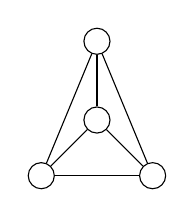
\begin{tikzpicture}[main/.style={draw,circle},node distance={1cm}]
                \node[main](0){};
                \node[main](1)[above of=0]{};
                \node[main](2)[below left of=0]{};
                \node[main](3)[below right of=0]{};
                \draw[-](0) -- (1);
                \draw[-](0) -- (2);
                \draw[-](0) -- (3);
                \draw[-](1) -- (2);
                \draw[-](1) -- (3);
                \draw[-](2) -- (3);
            \end{tikzpicture}
        \end{center}
    \end{eqbox} 
    
    \begin{definition}{Plane}{Graph}
        A \emph{plane} graph is a planar graph with a fixed planar embedding. We call vertices as \emph{points} and edges as \emph{lines}.
    \end{definition}
    
    \np A rigorous discussion of planarity involves topology, which is out of the scope of this note. But we shall take many topological results for granted. Moreover, we will mainly focus on the combinatorial aspects of planar graphs.

    \begin{recall}{Curve}{on a Topological Space}
        Let $X$ be a topological space. We say $C\subseteq X$ is a \emph{curve} on $X$ if there exists continuous $f:I\to X$ such that $C=\image\left( f \right)$, where $I\subseteq\R$ is an interval. We call $f$ a \emph{parameterization} of $C$.
    \end{recall}

    \begin{recall}{Simple, Closed, Jordan}{Curve}
        Let $C$ be a curve on a topological space $X$.
        \begin{enumerate}
            \item We say $C$ is \emph{simple} if it does not intersect itself, except at the endpoints.\footnote{Rigorously speaking, given a curve $C$ with a parameterization $f$ on an interval $I$, we say $C$ is simple if, for every $x,y\in I$, $f\left( x \right)=f\left( y \right)$ only if $x=y$ or $x,y$ are the endpoints of $I$.}
            \item We say $C$ is \emph{closed} if it is a continuous image of a unit circle.
            \item We say $C$ is \emph{Jordan} if $C$ is simple closed curve and $X=\R^{2}$.
        \end{enumerate}
    \end{recall}

    \begin{recall}{Connected}{Subset}
        Let $X$ be a topological space.
        \begin{enumerate}
            \item We say $X$ is \emph{disconnected} if $X$ is a union of two disjoint nonempty open subsets of $X$.
            \item We say $X$ is \emph{connected} if $X$ is not disconnected.
            \item A maximal connected subset of $X$ is called a \emph{connected component} of $X$.
        \end{enumerate}
    \end{recall}

    \begin{theorem}{Jordan Curve Theorem}
        Let $C$ be a Jordan curve. Then $\R^{2}\setminus C$ contains exactly $2$ connected components, one bounded and one unbounded.
    \end{theorem}

    \begin{recall}{Interior, Exterior}{of a Jordan Curve}
        Let $C$ be a Jordan curve.
        \begin{enumerate}
            \item The \emph{interior} of $C$, denoted as $\intr\left( C \right)$, is the bounded connected component of $\R^{2}\setminus C$.
            \item The \emph{exterior} of $C$, denoted as $\ext\left( C \right)$, is the unbounded connected component of $\R^{2}\setminus C$.
        \end{enumerate}
    \end{recall}

    \begin{cor}{}
        $K_5$ is not planar.
    \end{cor}

    \begin{proof}
        Suppose $K_5$ has a planar embedding for the sake of contradiction. Write $V\left( K_5 \right) = \left\lbrace v_1,v_2,v_3,v_4,v_5 \right\rbrace$. Then the lines
        \begin{equation*}
            v_1v_2,v_2v_3,v_3v_1
        \end{equation*}
        form a Jordan curve $C$, since $\left( \left\lbrace v_1,v_2,v_3 \right\rbrace, \left\lbrace v_1v_2,v_2v_3,v_3v_1 \right\rbrace \right)$ is a cycle in $K_5$. Then $v_4\in\intr\left( C \right)$ or $v_4\in\ext\left( C \right)$. Without loss of generality, assume $v_4\in\intr\left( C \right)$. Then the lines $v_4v_1,v_4v_2,v_4v_3$ are contained in $\int\left( C \right)$, execpt at $v_1,v_2,v_3$, respectively. Let $C_1,C_2,C_3$ be the Jordan curves formed by the cycles
        \begin{equation*}
            \left( \left\lbrace v_2,v_3,v_4 \right\rbrace, \left\lbrace v_2v_3,v_3v_4,v_4v_2 \right\rbrace \right), \left( \left\lbrace v_1,v_3,v_4 \right\rbrace, \left\lbrace v_1v_3,v_3v_4,v_4v_1 \right\rbrace \right), \left( \left\lbrace v_1,v_2,v_4 \right\rbrace, \left\lbrace v_1v_2,v_2v_4,v_4v_1 \right\rbrace \right),
        \end{equation*}
        respectively. Note that, for all $i\in\left\lbrace 1,2,3 \right\rbrace$, $\int\left( C_i \right)\subseteq\intr\left( C \right)$ and $v_i\in\ext\left( C \right)$. Since there is a line joining $v_5$ to $v_i$ for all $i\in\left\lbrace 1,2,3 \right\rbrace$, by the Jordan curve theorem $v_5\in\ext\left( C_i \right)$ for all $i\in\left\lbrace 1,2,3 \right\rbrace$. So $v_5\in\ext\left( C \right)$. But this contradicts the fact that $v_4\in\int\left( C \right)$ and $v_4,v_5$ are joined by a line. Thus $K_5$ is not planar.
    \end{proof}

    \begin{cor}{}
        $K_{3,3}$ is not planar.
    \end{cor}

    \begin{definition}{Subdivision}{of a Graph}
        Let $G$ be a graph. A \emph{subdivision} of $G$ is obtained from $G$ by replacing each edge with a new path of length at least $1$.
    \end{definition}
    
    \begin{prop}{}
        Let $G$ be a graph. The following are equivalent.
        \begin{enumerate}
            \item $G$ is planar.
            \item Every subdivision of $G$ is planar.
        \end{enumerate}
    \end{prop}

    \begin{proof}[Proof-ish]
        Note that an edge and a path are both represented by a simple curve.
    \end{proof}

    \clearpage
    \begin{cor}{}
        Any graph containing a subdivision of $K_5$ or $K_{3,3}$ is not planar.
    \end{cor}	
    
    
    
    
    
    
    
    
    
    
    
    
    
    
    
    
    
    
    
    
    
    
    
    
    
    
    
    
    
    
    
    
    
    
    
    
    
    
    
    
    
    

\end{document}
